\newpage
%\chapter*{Metodika měření a analýza výsledků} % normalni kapitola \chapter{kapitola}
%\addcontentsline{toc}{chapter}{Experimentální set-up a analýza výsledků}

\chapter{Metodika měření a analýza výsledků}

\textit{Anežka Kabátová}\\
V této kapitole bude popsáno, jak probíhalo měření pomocí experimentálního set-upu, který byl již částečně představen v předchozím textu. Bude vysvětleno, proč jsme přistoupili k jednotlivým řešením a s jakými problémy jsme se potýkali. Nakonec budou interpretovány výsledky měření thresholdu pro produkci charakteristického záření konverzní vrstvy, demonstrován pohyb svazku a proveden odhad energie měřených fotonů.\\

\section{Metodika měření}
Při výběru detekční technologie na úplném počátku našeho experimentu jsme se nejvíce obávali nedostatečné energie elektronového svazku, jelikož zvolený X-CHIP03 má na povrchu několik necitlivých vrstev, kterými nízkoenergetické částice neprojdou. Jelikož jsou ale pixelové křemíkové detektory velice perspektivní, rozhodli jsme se riskovat případné problémy za cenu vysokého přínosu naším dovednostem. Tato obava se bohužel vyplnila, protože ani přes opakovanou snahu dosáhnout vyšších energií se nepodařilo zabránit náhodným výbojům v komoře, které by mohly detektor zničit.\\
Abychom získali detekovatelné částice, rozhodli jsme se použít konverzní vrstvu ze slitiny mědi a zlata, která pomocí excitace a následné deexcitace atomů uvnitř ní vyzařuje charakteristické záření. Toto záření má samozřejmě maximálně stejnou energii, jako elektronový svazek, ale díky rozdílnému mechanismu interakce fotonů a elektronů s látkou nemají problém projít až do citlivé oblasti čipu. Použitím konverzní vrstvy jsme ale přišli o informaci o původní energii částic, jelikož po dosažení thresholdu se objeví charakteristické záření, jehož energie podléhá pouze statistickým fluktuacím. Na druhou stranu jsme získali přibližnou informaci o energii detekovaných částic, kterou jsme mohli dále využít pro kontrolu orientační kalibrace detekčního čipu.\\
Detekční čip je, jak už bylo zmíněno, složen z matice 4096 pixelů. Každý funguje jako samostatná detekční jednotka, skládající se z vyprázdněné oblasti, v níž dochází ke vzniku volných nosičů náboje, a vyčítacího obvodu, v němž se na základě Shockley-Ramo teorému generuje z pohybujícího se náboje proud. Výstupem celého obvodu jsou jednotky analogově digitálního převodníku (ADC jednotky). Ty mají s energií původní částice spojitost, jelikož množství volných nosičů náboje, tedy i proud, jsou na ní závislé. K přiřazení energetické škály konkrétnímu pixelu se však musí provézt časově náročná kalibrace.\\
Pro účely tohoto experimentu kalibrace provedena nebyla, ale byly využity kalibrační křivky stejného detektoru. Ověření správnosti tohoto odhadu nám poskytuje právě energie charakteristických fotonů.\\
Konverzní vrstva, jak už bylo zmíněno, byla slitina zlata a mědi, bohužel v neznámém poměru. Charakteristické rentgenové záření pro různé elektronové hladiny obsahuje Tab. \ref{Tabulka1}.

\begin{table}
\begin{tabular}{|c|c|c|c|c|c|c|c|c|c|}
     \hline 
     Prvek & K$\alpha_1$ & K$\alpha_2$ & K$\beta_1$ & L$\alpha_1$ & L$\alpha_2$ & L$\beta_1$ & L$\beta_2$ & L$\gamma_1$ & M$\alpha_1$ \\ 
     \hline 
     Cu & 8.0 & 8.0 & 8.9 & 0.9 & 0.9 & 0.9 & - & - & - \\ 
     \hline 
     Au & 68.8 & 67.0 & 78.0 & 9.7 & 9.6 & 11.4 & 11.6 & 13.4 & 2.1 \\ 
     \hline 
     \end{tabular}
     \caption{Energie charakteristického záření pro jednotlivé elektronové hladiny v keV pro zlato a meď.}   
     \label{Tabulka1}
     \end{table}   

\section{Postup měření}
Provedená měření je možné rozdělit na dvě skupiny. Nejprve byla testována fokusace, což bylo rozebráno v příslušné kapitole. Konverzní vrstva částečně smývá informaci o poloze svazku, jelikož emitované fotony nemají stejný směr pohybu, jako původní elektrony. Pro účely testování fokusace tedy tento set-up není vhodný, a byl proto dočasně z komory odstraněn.\\
Nalezení ideální polohy pro měření zobrazuje video v příloze. Vidíme, že množství detekovaných detektorů se skokově zvýšilo.\\
Důležité pro ověření konceptu konverzní vrstvy bylo nalezení thresholdu pro výskyt charakteristického záření, čemuž jsme se věnovali v druhé části experimentu.

\section{Výsledky}
Z dostupných dat pozorujeme, že k nárůstu střední hodnoty pixelů došlo, nicméně ostrý threshold patrný není. To může být způsobeno rozdílnou energií elektronů ve svazku. Rostoucí odezva čipu v závislosti na napětí elektrody je na Obr. \ref{Obrazek_threshold}.

\begin{figure}[htbp!]
\centering
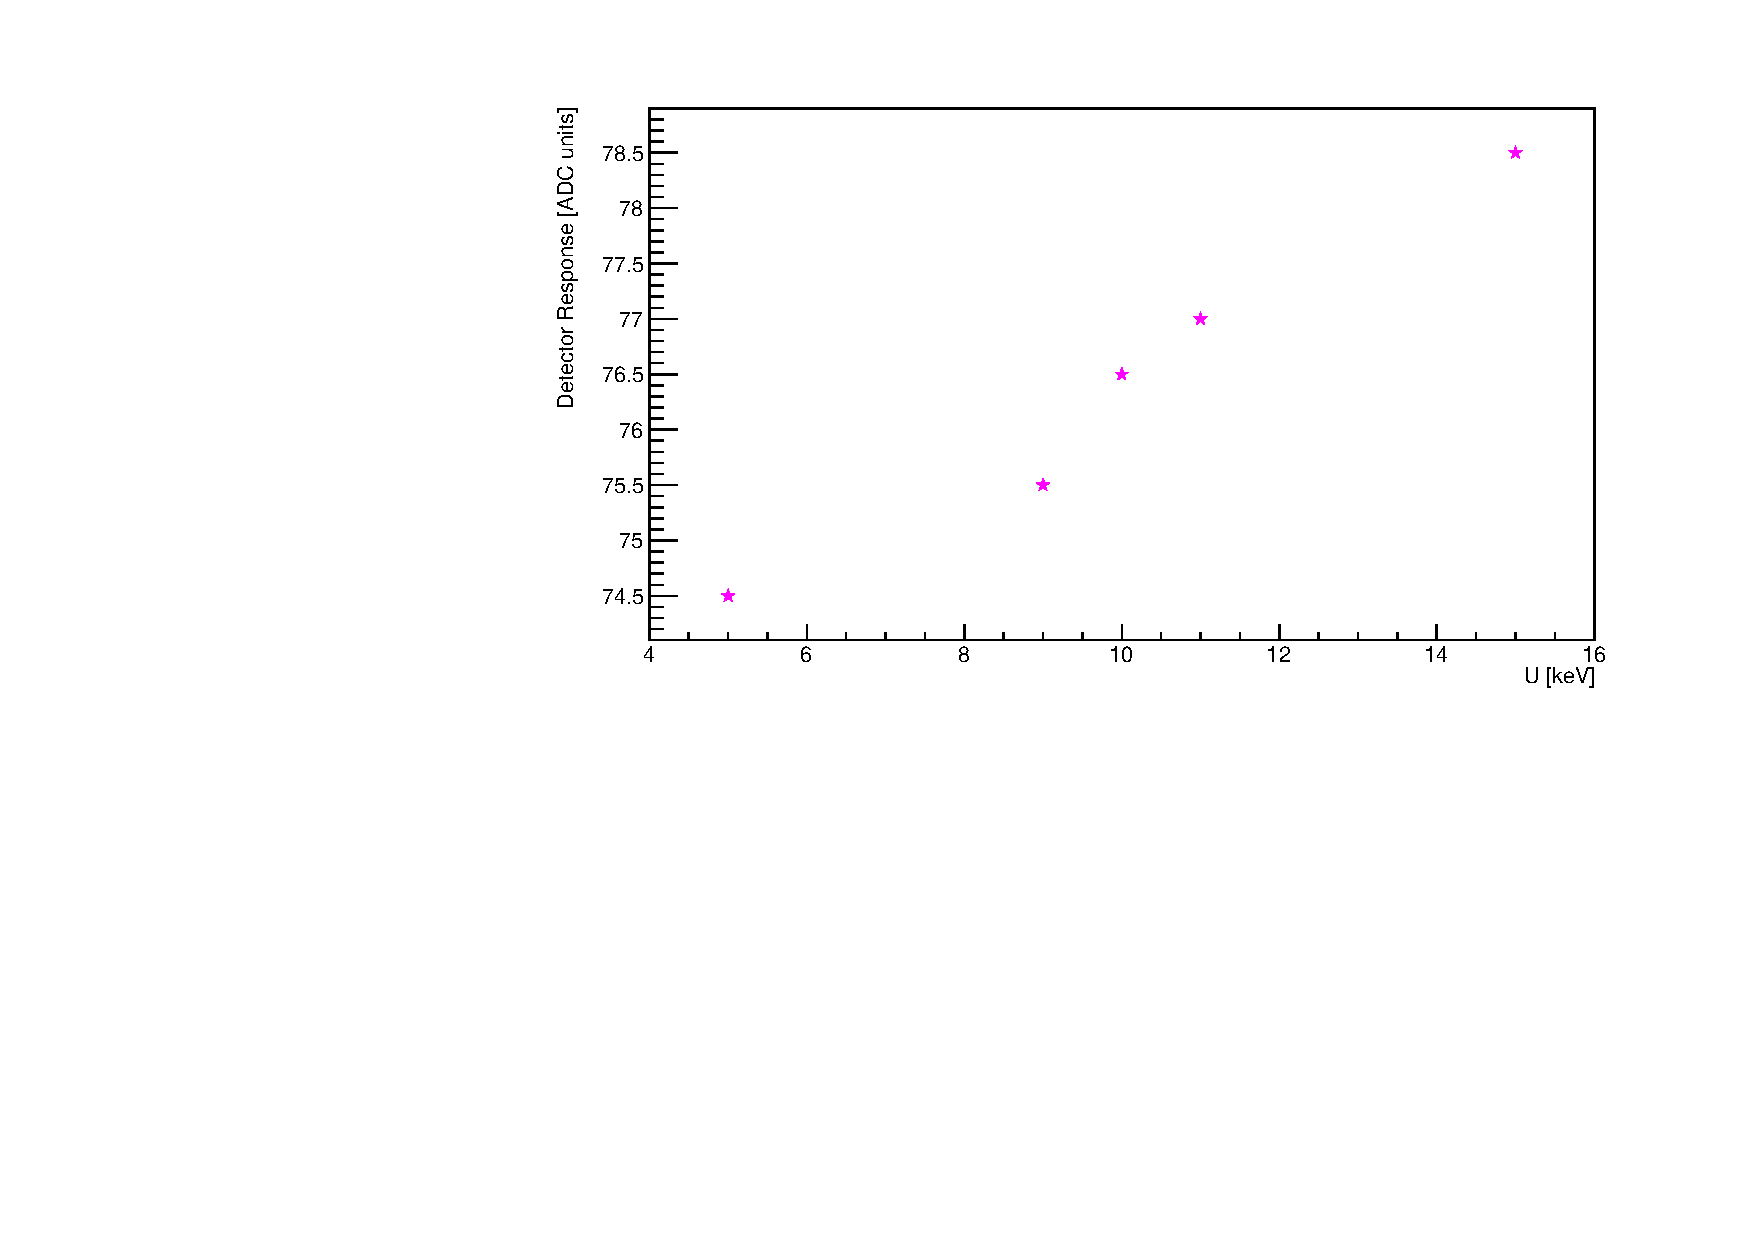
\includegraphics[scale = 0.7]{Figure/response.pdf}
 \caption{Střední odezva všech pixelů detektoru v jednotkách analogově-digitálního převodníku v závislosti na napětí elektrody elektronového děla.}
\label{Obrazek_threshold}
\end{figure}

Odezvu detektoru ve formě dvourozměrného histogramu lze najít na Obr. \ref{Obrazek_histo}. Souřadnicové osy odpovídají poloze jednotlivých pixelů v matici, jejich hodnota obsahuje informaci o střední odezvě daného pixelu.


\begin{figure}[htbp!]
\centering
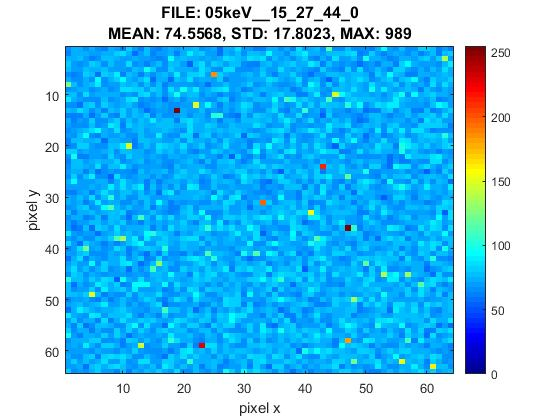
\includegraphics[width = 200 pt]{Figure/100_05keV__15_27_44_0.jpg}
\hfill
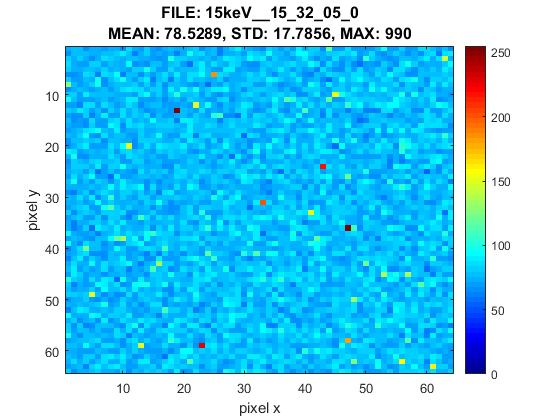
\includegraphics[width = 200 pt]{Figure/100_15keV__15_32_05_0.jpg}
 \caption{Dvourozměrné histogramy zobrazující momentální odezvu čipu pro nízké a vysoké napětí elektrody děla.}
\label{Obrazek_histo}
\end{figure}

Pomocí tohoto typu histogramu bylo také zjištěno, jaká byla přibližně energie detekovaných fotonů. Na detektoru stejného typu byla provedena energetická kalibrace jednotlivých pixelů, kterou lze využít k tomuto odhadu. Jak už bylo zmíněno, každý pixel v matici je svým způsobem originální kvůli nedokonalému výrobnímu procesu, jemuž se nedá předejít. Proto je třeba každému individuálnímu obvodu přiřadit lineární vztah mezi odezvou v ADC jednotkách a skutečnou energií. Dělá se tak pomocí známých spekter, jako jsou železo nebo plutonium. Nejprve jsou změřeny píky těchto spekter pomocí kalibrovaného detektoru, poté je jim přiřazena správná hodnota. Pokud je změřených píků dost, v tomto případě 4 (spektrum železa má jeden rozlišitelný pík, plutonium tři), lze těmito body proložit křivka a získat tak kýžený vztah.\\
Kalibrační křivku vybraného pixelu pro několik teplotních bodů zobrazuje Obr. \ref{Obrazek_kalibrace}.

 \begin{figure}[htbp!]
\centering
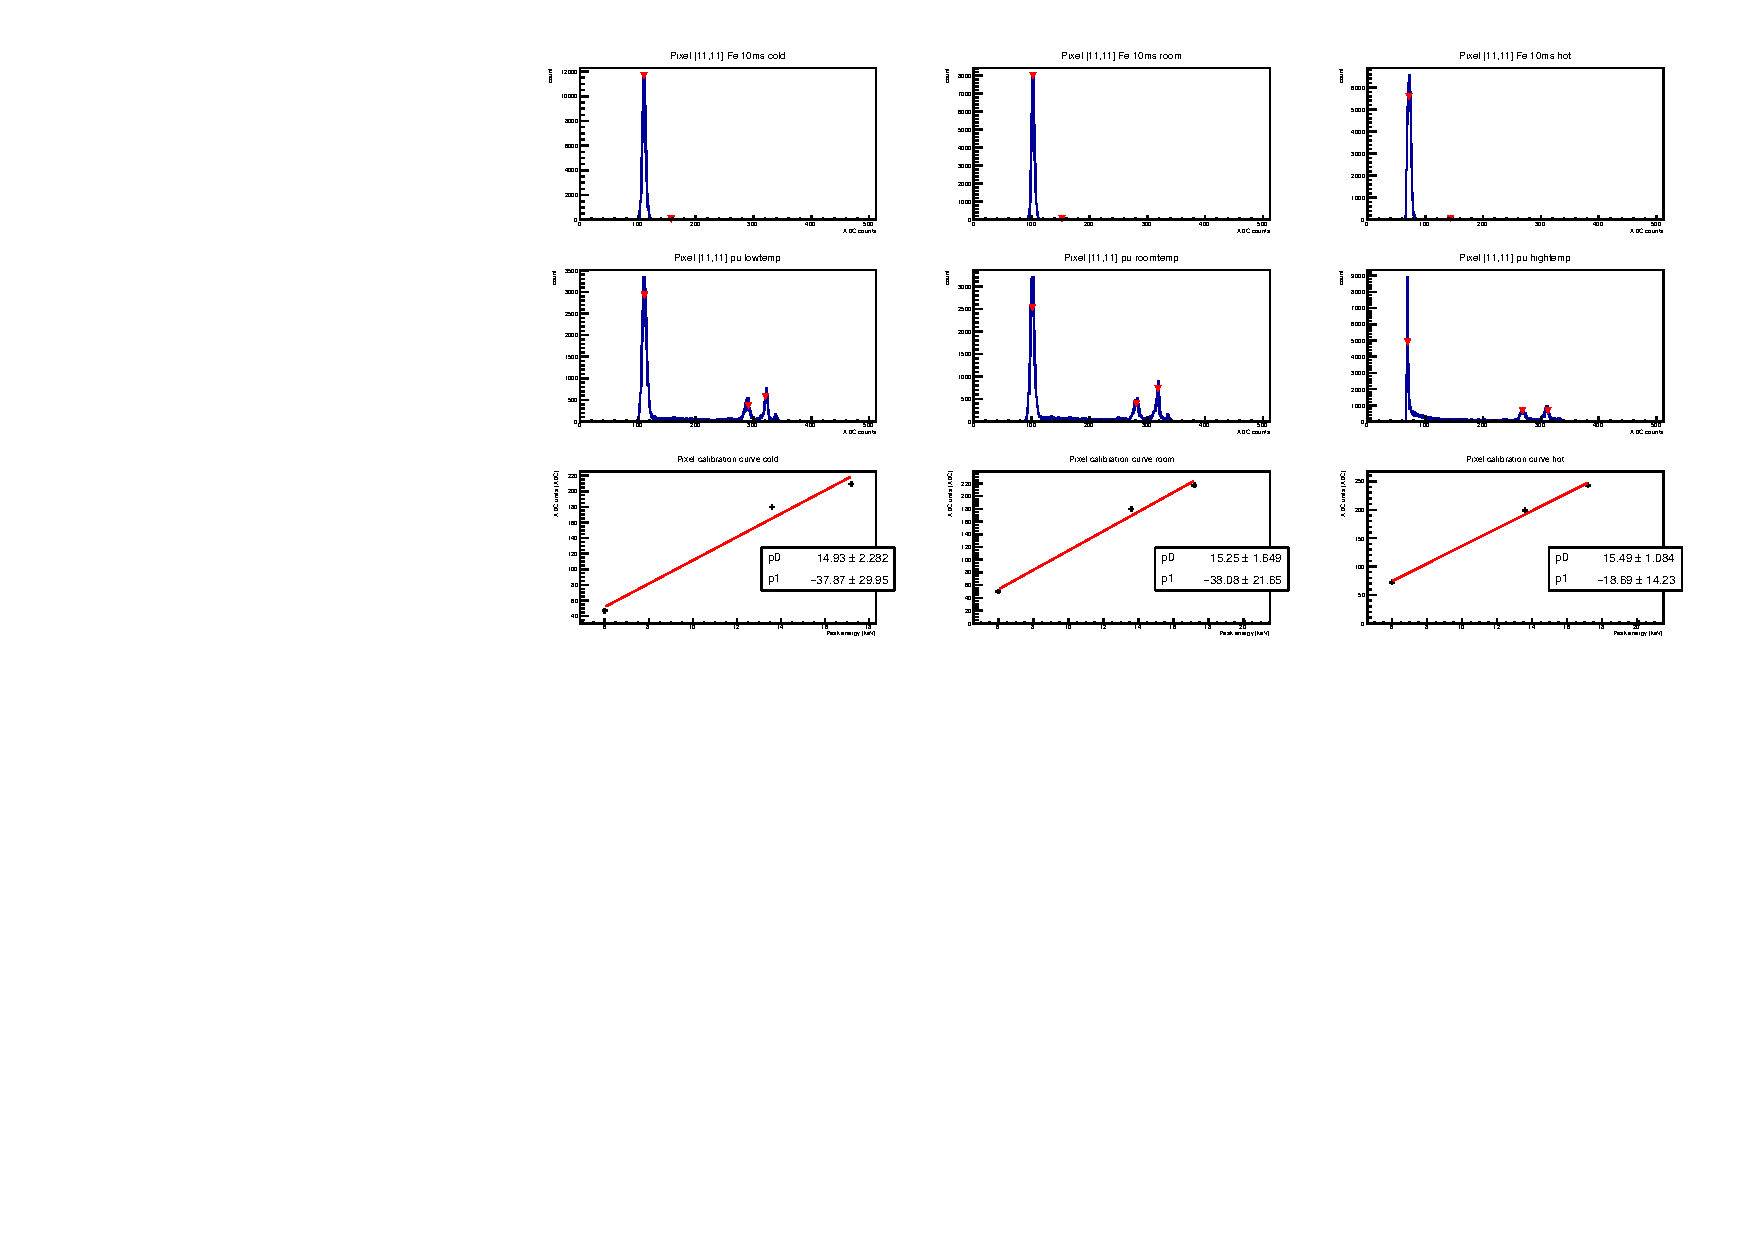
\includegraphics[scale = 0.85]{Figure/calibration.pdf}
 \caption{Kalibrace pixelu 11,11. Obrázky v prvních dvou řádcích zobrazují změřená spektra a v nich nalezené píky. V tomto případě byly pro kalibraci použity dva píky plutonia a jeden pík železa změřené při teplotě kolem 0$^{\circ}$, pokojové teplotě a teplotě kolem 60$^{\circ}$. Trojice obrázků ve spodním řádku pak zobrazuje kalibrační křivky a jejich parametry.}
\label{Obrazek_kalibrace}
\end{figure}

Pozorovaný rozdíl v ADC jednotkách mezi odezvou pixelu zasaženého elektronem a pozadím byl přibližně 80 ADC jednotek, což odpovídá podle kalibrační křivky zhruba 8 keV. To je v souladu s očekáváním, jelikož charakteristickému spektru mědi dominují fotony ze slupek K, které mají energii okolo 8 keV. 

 \begin{figure}[htbp!]
\centering
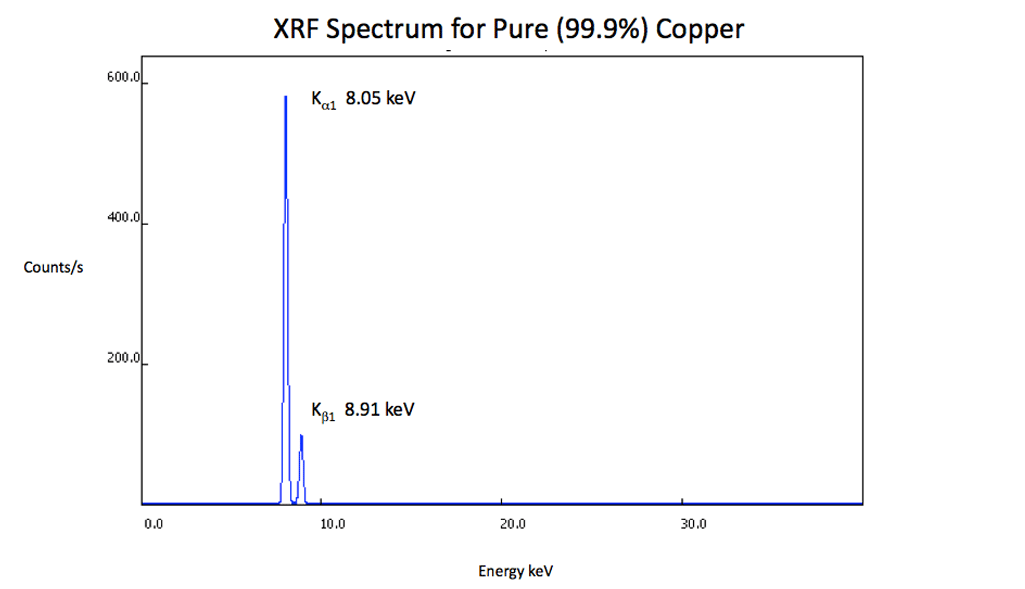
\includegraphics[scale = 0.4]{Figure/spektrum.png}
 \caption{Spektrum mědi s charakteristickými píky odpovídajícími fotonům emitovaných při deexcitaci na dvě vnitřní K-slupky.}
\end{figure}

